\documentclass[12pt]{beamer}\usepackage[]{graphicx}\usepackage[]{color}
%% maxwidth is the original width if it is less than linewidth
%% otherwise use linewidth (to make sure the graphics do not exceed the margin)
\makeatletter
\def\maxwidth{ %
  \ifdim\Gin@nat@width>\linewidth
    \linewidth
  \else
    \Gin@nat@width
  \fi
}
\makeatother

\definecolor{fgcolor}{rgb}{0.345, 0.345, 0.345}
\newcommand{\hlnum}[1]{\textcolor[rgb]{0.686,0.059,0.569}{#1}}%
\newcommand{\hlstr}[1]{\textcolor[rgb]{0.192,0.494,0.8}{#1}}%
\newcommand{\hlcom}[1]{\textcolor[rgb]{0.678,0.584,0.686}{\textit{#1}}}%
\newcommand{\hlopt}[1]{\textcolor[rgb]{0,0,0}{#1}}%
\newcommand{\hlstd}[1]{\textcolor[rgb]{0.345,0.345,0.345}{#1}}%
\newcommand{\hlkwa}[1]{\textcolor[rgb]{0.161,0.373,0.58}{\textbf{#1}}}%
\newcommand{\hlkwb}[1]{\textcolor[rgb]{0.69,0.353,0.396}{#1}}%
\newcommand{\hlkwc}[1]{\textcolor[rgb]{0.333,0.667,0.333}{#1}}%
\newcommand{\hlkwd}[1]{\textcolor[rgb]{0.737,0.353,0.396}{\textbf{#1}}}%
\let\hlipl\hlkwb

\usepackage{framed}
\makeatletter
\newenvironment{kframe}{%
 \def\at@end@of@kframe{}%
 \ifinner\ifhmode%
  \def\at@end@of@kframe{\end{minipage}}%
  \begin{minipage}{\columnwidth}%
 \fi\fi%
 \def\FrameCommand##1{\hskip\@totalleftmargin \hskip-\fboxsep
 \colorbox{shadecolor}{##1}\hskip-\fboxsep
     % There is no \\@totalrightmargin, so:
     \hskip-\linewidth \hskip-\@totalleftmargin \hskip\columnwidth}%
 \MakeFramed {\advance\hsize-\width
   \@totalleftmargin\z@ \linewidth\hsize
   \@setminipage}}%
 {\par\unskip\endMakeFramed%
 \at@end@of@kframe}
\makeatother

\definecolor{shadecolor}{rgb}{.97, .97, .97}
\definecolor{messagecolor}{rgb}{0, 0, 0}
\definecolor{warningcolor}{rgb}{1, 0, 1}
\definecolor{errorcolor}{rgb}{1, 0, 0}
\newenvironment{knitrout}{}{} % an empty environment to be redefined in TeX

\usepackage{alltt}
\usepackage{graphicx}
\usepackage{tikz}
\setbeameroption{hide notes}
\setbeamertemplate{note page}[plain]
\usepackage{listings}

% get rid of junk
\usetheme{default}
\usefonttheme[onlymath]{serif}
\beamertemplatenavigationsymbolsempty
\hypersetup{pdfpagemode=UseNone} % don't show bookmarks on initial view

% named colors
\definecolor{offwhite}{RGB}{255,250,240}
\definecolor{gray}{RGB}{155,155,155}

\ifx\notescolors\undefined % slides

  \definecolor{foreground}{RGB}{80,80,80}
  \definecolor{background}{RGB}{255,255,255}
  \definecolor{title}{RGB}{255,199,0}
  \definecolor{subtitle}{RGB}{89,132,212}
  \definecolor{hilit}{RGB}{248,117,79}
  \definecolor{vhilit}{RGB}{255,111,207}
  \definecolor{lolit}{RGB}{200,200,200}
  \definecolor{lit}{RGB}{255,199,0}
  \definecolor{mdlit}{RGB}{89,132,212}
  \definecolor{link}{RGB}{248,117,79}

\else % notes
  \definecolor{background}{RGB}{255,255,255}
  \definecolor{foreground}{RGB}{24,24,24}
  \definecolor{title}{RGB}{27,94,134}
  \definecolor{subtitle}{RGB}{22,175,124}
  \definecolor{hilit}{RGB}{122,0,128}
  \definecolor{vhilit}{RGB}{255,0,128}
  \definecolor{lolit}{RGB}{95,95,95}
\fi
\definecolor{nhilit}{RGB}{128,0,128}  % hilit color in notes
\definecolor{nvhilit}{RGB}{255,0,128} % vhilit for notes

\newcommand{\hilit}{\color{hilit}}
\newcommand{\vhilit}{\color{vhilit}}
\newcommand{\nhilit}{\color{nhilit}}
\newcommand{\nvhilit}{\color{nvhilit}}
\newcommand{\lit}{\color{lit}}
\newcommand{\mdlit}{\color{mdlit}}
\newcommand{\lolit}{\color{lolit}}

% use those colors
\setbeamercolor{titlelike}{fg=title}
\setbeamercolor{subtitle}{fg=subtitle}
\setbeamercolor{frametitle}{fg=gray}
\setbeamercolor{structure}{fg=subtitle}
\setbeamercolor{institute}{fg=lolit}
\setbeamercolor{normal text}{fg=foreground,bg=background}
%\setbeamercolor{item}{fg=foreground} % color of bullets
%\setbeamercolor{subitem}{fg=hilit}
%\setbeamercolor{itemize/enumerate subbody}{fg=lolit}
\setbeamertemplate{itemize subitem}{{\textendash}}
\setbeamerfont{itemize/enumerate subbody}{size=\footnotesize}
\setbeamerfont{itemize/enumerate subitem}{size=\footnotesize}

% center title of slides
\setbeamertemplate{blocks}[rounded]
\setbeamertemplate{frametitle}[default][center]
% margins
\setbeamersize{text margin left=25pt,text margin right=25pt}

% page number
\setbeamertemplate{footline}{%
    \raisebox{5pt}{\makebox[\paperwidth]{\hfill\makebox[20pt]{\lolit
          \scriptsize\insertframenumber}}}\hspace*{5pt}}

% add a bit of space at the top of the notes page
\addtobeamertemplate{note page}{\setlength{\parskip}{12pt}}

% default link color
\hypersetup{colorlinks, urlcolor={link}}

\ifx\notescolors\undefined % slides
  % set up listing environment
  \lstset{language=bash,
          basicstyle=\ttfamily\scriptsize,
          frame=single,
          commentstyle=,
          backgroundcolor=\color{darkgray},
          showspaces=false,
          showstringspaces=false
          }
\else % notes
  \lstset{language=bash,
          basicstyle=\ttfamily\scriptsize,
          frame=single,
          commentstyle=,
          backgroundcolor=\color{offwhite},
          showspaces=false,
          showstringspaces=false
          }
\fi

% a few macros
\newcommand{\code}[1]{\texttt{#1}}
\newcommand{\hicode}[1]{{\hilit \texttt{#1}}}
\newcommand{\bb}[1]{\begin{block}{#1}}
\newcommand{\eb}{\end{block}}
\newcommand{\bi}{\begin{itemize}}
%\newcommand{\bbi}{\vspace{24pt} \begin{itemize} \itemsep8pt}
\newcommand{\bbi}{\vspace{4pt} \begin{itemize} \itemsep8pt}
\newcommand{\ei}{\end{itemize}}
\newcommand{\bv}{\begin{verbatim}}
\newcommand{\ev}{\end{verbatim}}
\newcommand{\ig}{\includegraphics}
\newcommand{\subt}[1]{{\footnotesize \color{subtitle} {#1}}}
\newcommand{\ttsm}{\tt \small}
\newcommand{\ttfn}{\tt \footnotesize}
\newcommand{\figh}[2]{\centerline{\includegraphics[height=#2\textheight]{#1}}}
\newcommand{\figw}[2]{\centerline{\includegraphics[width=#2\textwidth]{#1}}}



%------------------------------------------------
% end of header
%------------------------------------------------

\title{Graphics in R}
\subtitle{STAT 133}
\author{\href{http://www.gastonsanchez.com}{Gaston Sanchez}}
\institute{\href{https://github.com/ucb-stat133/stat133-fall-2016}{\tt \scriptsize \color{foreground} github.com/ucb-stat133/stat133-fall-2016}}
\date{}
\IfFileExists{upquote.sty}{\usepackage{upquote}}{}
\begin{document}


{
  \setbeamertemplate{footline}{} % no page number here
  \frame{
    \titlepage
  } 
}

%------------------------------------------------

\begin{frame}
\begin{center}
\Huge{\hilit{R Graphics}}
\end{center}
\end{frame}

%------------------------------------------------

\begin{frame}
\frametitle{Understanding Graphics in R}

\centerline{\mdlit \Large 2 main graphics systems}

\bigskip
\centerline{\Large \code{"graphics"} \quad \& \quad \code{"grid"}}

\end{frame}

%------------------------------------------------

\begin{frame}
\frametitle{Basics of Graphics in R}

\bb{Graphics Systems}
\bbi
  \item \code{"graphics"} and \code{"grid"} are the two main graphics systems in R
  \item \code{"graphics"} is the \textit{traditional} system, also referred to as \textit{base graphics}
  \item \code{"grid"} prodives low-level functions for programming plotting functions
\ei
\eb

\end{frame}

%------------------------------------------------

\begin{frame}
\frametitle{Basics of Graphics in R}

\bb{Graphics Engine}
\bbi
  \item Underneath \code{"graphics"} and \code{"grid"} there is the package \code{"grDevices"}
  \item \code{"grDevices"} is the graphics \textbf{engine} in R
  \item It provides the graphics devices and support for colors and fonts
\ei
\eb

\end{frame}

%------------------------------------------------

\begin{frame}[fragile]
\begin{center}
\ig[width=8cm]{images/graphic_systems.pdf}
\end{center}
\end{frame}

%------------------------------------------------

\begin{frame}
\frametitle{Basics of Graphics in R}

\bb{Package \code{"graphics"}}
The package \code{"graphics"} is the traditional system; it provides functions for complete plots, as well as low-level facilities. 

\bigskip
Many other graphics packages are built on top of graphics like \code{"maps"}, \code{"diagram"}, \code{"pixmap"}, and many more.
\eb

\end{frame}

%------------------------------------------------

\begin{frame}
\frametitle{Understanding Graphics in R}

\bb{Package \code{"grid"}}
The \code{"grid"} package does not provide functions for drawing complete plots.

\bigskip
\code{"grid"} is not used directly to produce statistical plots. Instead, it is used to build other graphics packages like \code{"lattice"} or \code{"ggplot2"}.
\eb

\end{frame}

%------------------------------------------------

\begin{frame}
\frametitle{In this course}

\bbi
 \item In this course we'll focus on the packages {\hilit \code{"graphics"}} and {\hilit \code{"ggplot2"}}
 \item \code{"graphics"} is the traditional plotting system in R, and many functions and packages are built on top of it.
 \item \code{"ggplot2"} excels at providing graphics for visualizing multivariate data sets ---in \code{data.frame} format---, while taking care of many issues for superior visual displays.
\ei

\end{frame}

%------------------------------------------------

\begin{frame}
\frametitle{R Graphics by Paul Murrell}
\begin{center}
\ig[height=6cm]{images/rgraphics.jpg}
\end{center}
\end{frame}

%------------------------------------------------

\begin{frame}
\frametitle{Some Resources}

\bi
 \item \textbf{R Graphics} by Paul Murrell \\
 \href{http://lux.e-reading.bz/bookreader.php/137370/C486x_C02.pdf}{\tt book} and \href{https://www.stat.auckland.ac.nz/~paul/RG2e/}{webpage}
 \item \textbf{R Graphics Cookbook} by Winston Chang \\
 \url{http://www.cookbook-r.com/Graphs/}
 \item \textbf{ggplot2: Elegant Graphics for Data Analysis} by Hadley Wickham
 \item \textbf{R Graphs Cookbook} by Hrishi Mittal
 \item \textbf{Graphics for Statistics and Data Analysis with R} by Kevin Keen
\ei

\end{frame}

%------------------------------------------------

\begin{frame}
\begin{center}
\Huge{\hilit{Traditional (Base) Graphics}}
\end{center}
\end{frame}

%------------------------------------------------

\begin{frame}
\frametitle{Base Graphics in R}

\bb{Types of graphics functions}
Graphics functions can be divided into two main types:
 \bi
  \item \textbf{high-level} functions produce complete plots, e.g. {\lit \code{barplot(), boxplot(), dotchart()}}
  \item \textbf{low-level} functions add further output to an existing plot, e.g. {\lit \code{text(), points(), legend()}}
 \ei
\eb

\end{frame}

%------------------------------------------------

\begin{frame}
\frametitle{The \code{plot()} function}

\bi
 \item {\hilit \code{plot()}} is the most important high-level function in traditional graphics
 \item The first argument to \code{plot()} provides the data to plot
 \item The provided data can take different forms: e.g. vectors, factors, matrices, data frames.
 \item To be more precise, \code{plot()} is a generic function
 \item You can create your own \code{plot()} method function
\ei

\end{frame}

%------------------------------------------------

\begin{frame}
\frametitle{Basic Plots with \code{plot()}}

In its basic form, we can use {\hilit \code{plot()}} to make graphics of:
\bi
  \item one single variable
  \item two variables
  \item multiple variables
\ei

\end{frame}

%------------------------------------------------

\begin{frame}
\begin{center}
\Huge{\hilit{Plots of One Variable}}
\end{center}
\end{frame}

%------------------------------------------------

\begin{frame}
\frametitle{High-level graphics of a single variable}

\begin{center}
 \begin{tabular}{l l l}
  \hline
   Function & Data & Description \\
  \hline
  \code{plot()} & numeric & scatterplot \\  
  \code{plot()} & factor & barplot \\
  \code{plot()} & 1-D table & barplot \\
  \hline
 \end{tabular}
\end{center}

\code{numeric} can be either a vector or a 1-D array (e.g. row or column from a matrix) 
\end{frame}

%------------------------------------------------

\begin{frame}
\frametitle{One variable objects}
\begin{center}
\ig[width=8cm]{images/one_variable_objs.pdf}
\end{center}
\end{frame}

%------------------------------------------------

\begin{frame}[fragile]
\frametitle{\code{plot()} of one variable}
\begin{knitrout}\footnotesize
\definecolor{shadecolor}{rgb}{0.969, 0.969, 0.969}\color{fgcolor}\begin{kframe}
\begin{alltt}
\hlcom{# plot numeric vector}
\hlstd{num_vec} \hlkwb{<-} \hlstd{(}\hlkwd{c}\hlstd{(}\hlnum{1}\hlopt{:}\hlnum{10}\hlstd{))}\hlopt{^}\hlnum{2}
\hlkwd{plot}\hlstd{(num_vec)}

\hlcom{# plot factor}
\hlkwd{set.seed}\hlstd{(}\hlnum{4}\hlstd{)}
\hlstd{abc} \hlkwb{<-} \hlkwd{factor}\hlstd{(}\hlkwd{sample}\hlstd{(}\hlkwd{c}\hlstd{(}\hlstr{'A'}\hlstd{,} \hlstr{'B'}\hlstd{,} \hlstr{'C'}\hlstd{),} \hlnum{20}\hlstd{,} \hlkwc{replace} \hlstd{=} \hlnum{TRUE}\hlstd{))}
\hlkwd{plot}\hlstd{(abc)}

\hlcom{# plot 1D-table}
\hlstd{abc_table} \hlkwb{<-} \hlkwd{table}\hlstd{(abc)}
\hlkwd{plot}\hlstd{(abc_table)}
\end{alltt}
\end{kframe}
\end{knitrout}
\end{frame}

%------------------------------------------------

\begin{frame}[fragile]
\frametitle{\code{plot()} of one variable}
\begin{knitrout}\footnotesize
\definecolor{shadecolor}{rgb}{0.969, 0.969, 0.969}\color{fgcolor}

{\centering 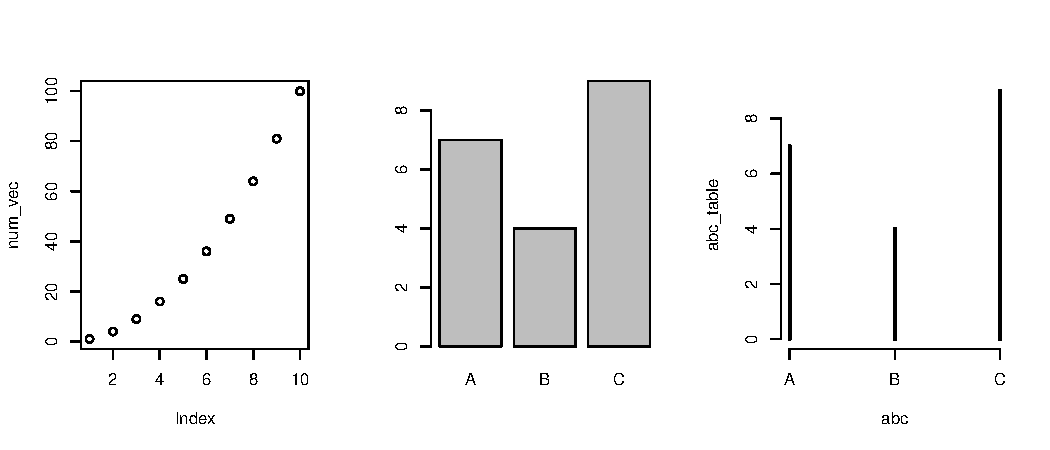
\includegraphics[width=.9\linewidth,height=.5\linewidth]{figure/plot_single1-1} 

}



\end{knitrout}
\end{frame}

%------------------------------------------------

\begin{frame}
\frametitle{More high-level graphics of a single variable}

\begin{center}
 \begin{tabular}{l l l}
  \hline
   Function & Data & Description \\
  \hline
  \code{barplot()} & numeric & barplot \\
  \code{pie()} & numeric & pie chart  \\
  \code{dotchart()} & numeric & dotplot \\
   & & \\
  \code{boxplot()} & numeric & boxplot \\
  \code{hist()} & numeric & histogram  \\
  \code{stripchart()} & numeric & 1-D scatterplot \\
  \code{stem()} & numeric & stem-and-leaf plot \\
  \hline
 \end{tabular}
\end{center}

\end{frame}

%------------------------------------------------

\begin{frame}[fragile]
\frametitle{Plots of one variable}
\begin{knitrout}\footnotesize
\definecolor{shadecolor}{rgb}{0.969, 0.969, 0.969}\color{fgcolor}\begin{kframe}
\begin{alltt}
\hlcom{# barplot numeric vector}
\hlkwd{barplot}\hlstd{(num_vec)}

\hlcom{# pie chart}
\hlkwd{pie}\hlstd{(}\hlnum{1}\hlopt{:}\hlnum{3}\hlstd{)}

\hlcom{# dot plot}
\hlkwd{dotchart}\hlstd{(num_vec)}
\end{alltt}
\end{kframe}
\end{knitrout}
\end{frame}

%------------------------------------------------

\begin{frame}[fragile]
\frametitle{Plots of one variable}
\begin{knitrout}\footnotesize
\definecolor{shadecolor}{rgb}{0.969, 0.969, 0.969}\color{fgcolor}

{\centering 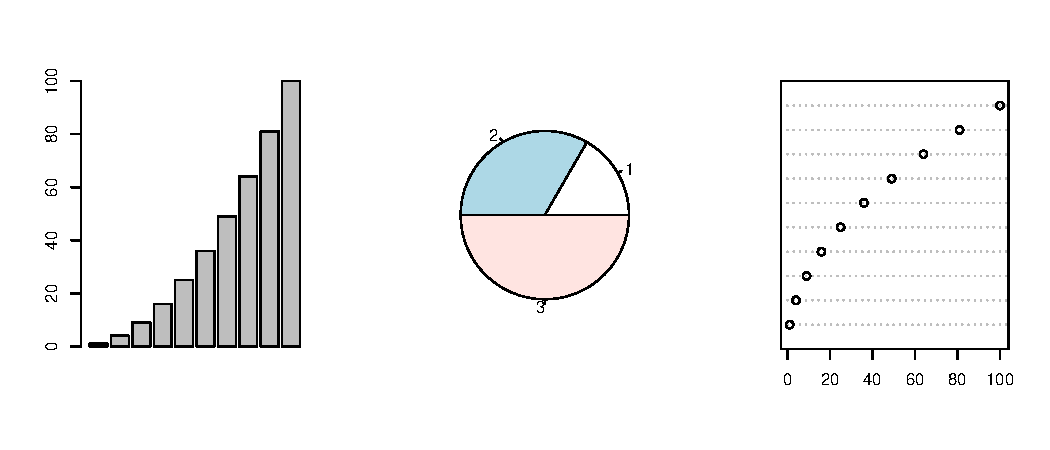
\includegraphics[width=.95\linewidth,height=.5\linewidth]{figure/plot_single2-1} 

}



\end{knitrout}
\end{frame}

%------------------------------------------------

\begin{frame}[fragile]
\frametitle{Plots of one variable}
\begin{knitrout}\footnotesize
\definecolor{shadecolor}{rgb}{0.969, 0.969, 0.969}\color{fgcolor}\begin{kframe}
\begin{alltt}
\hlcom{# barplot numeric vector}
\hlkwd{boxplot}\hlstd{(num_vec)}

\hlcom{# pie chart}
\hlkwd{hist}\hlstd{(num_vec)}

\hlcom{# dot plot}
\hlkwd{stripchart}\hlstd{(num_vec)}

\hlcom{# stem-and-leaf}
\hlkwd{stem}\hlstd{(num_vec)}
\end{alltt}
\end{kframe}
\end{knitrout}
\end{frame}

%------------------------------------------------

\begin{frame}[fragile]
\frametitle{\code{boxplot()}}
\begin{knitrout}\footnotesize
\definecolor{shadecolor}{rgb}{0.969, 0.969, 0.969}\color{fgcolor}\begin{kframe}
\begin{alltt}
\hlcom{# boxplot}
\hlkwd{boxplot}\hlstd{(iris}\hlopt{$}\hlstd{Sepal.Length)}
\end{alltt}
\end{kframe}

{\centering 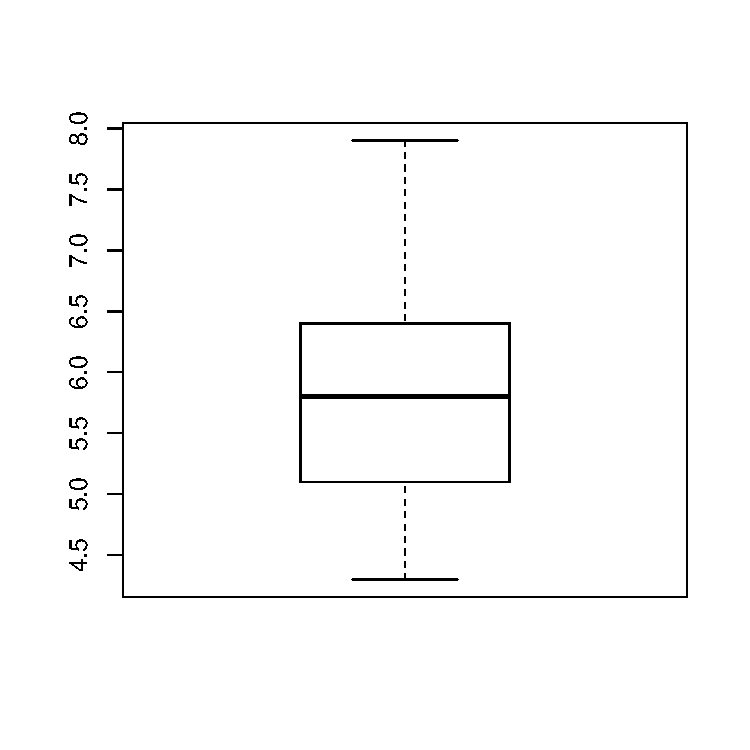
\includegraphics[width=.5\linewidth,height=.5\linewidth]{figure/unnamed-chunk-1-1} 

}



\end{knitrout}
\end{frame}

%------------------------------------------------

\begin{frame}[fragile]
\frametitle{\code{hist()}}
\begin{knitrout}\footnotesize
\definecolor{shadecolor}{rgb}{0.969, 0.969, 0.969}\color{fgcolor}\begin{kframe}
\begin{alltt}
\hlcom{# histogram}
\hlkwd{hist}\hlstd{(iris}\hlopt{$}\hlstd{Sepal.Length)}
\end{alltt}
\end{kframe}

{\centering 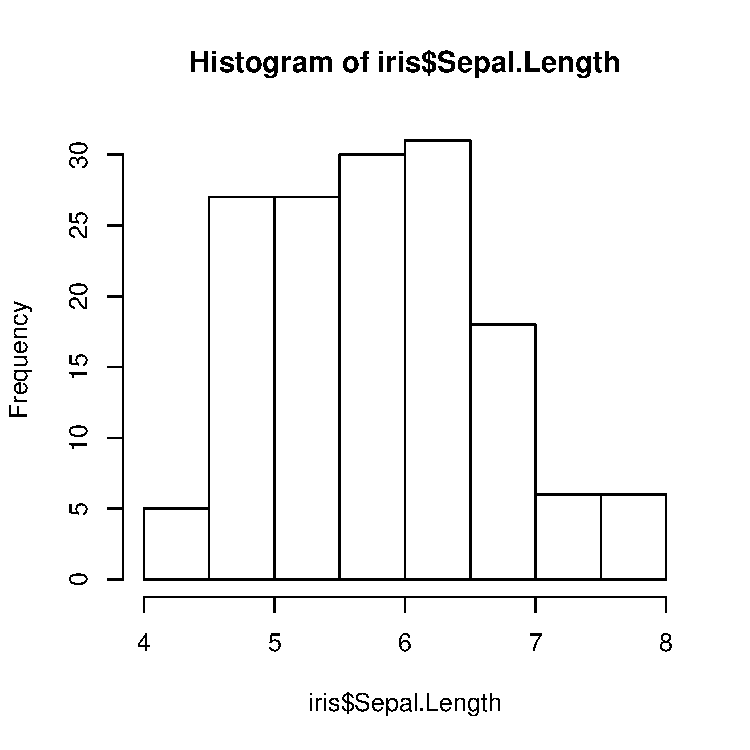
\includegraphics[width=.5\linewidth,height=.5\linewidth]{figure/unnamed-chunk-2-1} 

}



\end{knitrout}
\end{frame}

%------------------------------------------------

\begin{frame}
\frametitle{Test your knowledge}

\bb{What option does not apply to histograms:}
\bbi
  \item[A)] adjacent bars (no gaps)
  \item[B)] area of bars indicate proportions
  \item[C)] bins of equal length
  \item[D)] bars can be reordered
\ei
\eb

\end{frame}

%------------------------------------------------

\begin{frame}[fragile]
\frametitle{\code{stripchart()}}
\begin{knitrout}\footnotesize
\definecolor{shadecolor}{rgb}{0.969, 0.969, 0.969}\color{fgcolor}\begin{kframe}
\begin{alltt}
\hlcom{# strip-chart (1-D scatter plot)}
\hlcom{# (for small sample sizes)}
\hlkwd{stripchart}\hlstd{(num_vec)}
\end{alltt}
\end{kframe}

{\centering 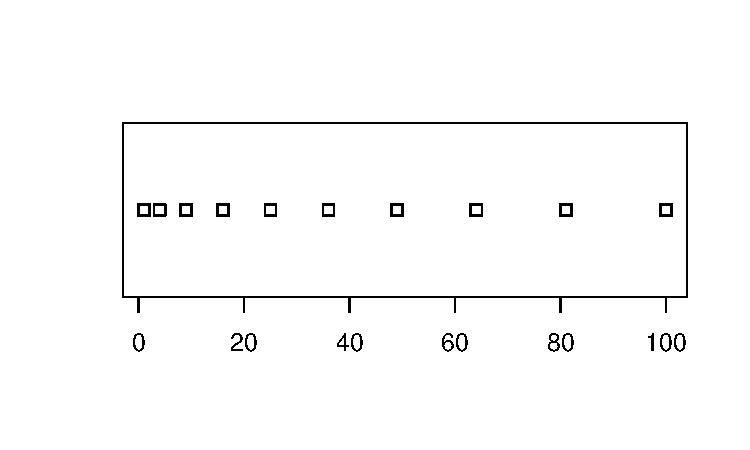
\includegraphics[width=.8\linewidth,height=.5\linewidth]{figure/unnamed-chunk-3-1} 

}



\end{knitrout}
\end{frame}

%------------------------------------------------

\begin{frame}[fragile]
\frametitle{\code{stem()}}
\begin{knitrout}\footnotesize
\definecolor{shadecolor}{rgb}{0.969, 0.969, 0.969}\color{fgcolor}\begin{kframe}
\begin{alltt}
\hlcom{# stem-and-leaf plot}
\hlcom{# (for small sample sizes)}
\hlkwd{stem}\hlstd{(num_vec)}
\end{alltt}
\begin{verbatim}
## 
##   The decimal point is 1 digit(s) to the right of the |
## 
##    0 | 1496
##    2 | 56
##    4 | 9
##    6 | 4
##    8 | 1
##   10 | 0
\end{verbatim}
\end{kframe}
\end{knitrout}
\end{frame}

%------------------------------------------------

\begin{frame}
\frametitle{Kernel Density Curve}

\bbi
  \item Surprisingly, R does not have a specific function to plot density curves
  \item R does have the \code{density()} function which computes a kernel density estimate
  \item We can pass a \code{"density"} object to \code{plot()} in order to get a density curve.
\ei

\end{frame}

%------------------------------------------------

\begin{frame}[fragile]
\frametitle{Kernel Density Curve}
\begin{knitrout}\footnotesize
\definecolor{shadecolor}{rgb}{0.969, 0.969, 0.969}\color{fgcolor}\begin{kframe}
\begin{alltt}
\hlcom{# kernel density curve}
\hlstd{dens} \hlkwb{<-} \hlkwd{density}\hlstd{(num_vec)}
\hlkwd{plot}\hlstd{(dens)}
\end{alltt}
\end{kframe}

{\centering 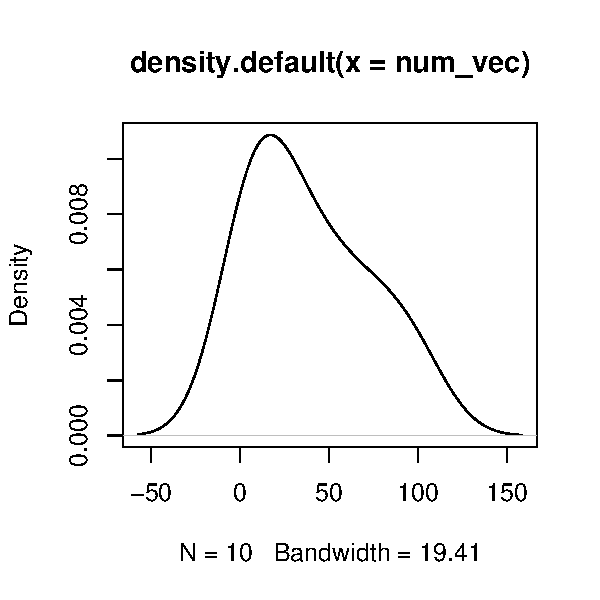
\includegraphics[width=.5\linewidth,height=.5\linewidth]{figure/unnamed-chunk-5-1} 

}



\end{knitrout}
\end{frame}

%------------------------------------------------

\begin{frame}
\frametitle{Test your knowledge}

\bb{What type of plot is based on the five-number summary}
\bbi
  \item[A)] bar chart
  \item[B)] box plot
  \item[C)] histogram
  \item[D)] scatterplot
\ei
\eb

\end{frame}

%------------------------------------------------

\begin{frame}
\begin{center}
\Huge{\hilit{Plots of Two Variables}}
\end{center}
\end{frame}

%------------------------------------------------

\begin{frame}
\frametitle{High-level graphics of two variables}

\begin{center}
 \begin{tabular}{l l l}
  \hline
   Function & Data & Description \\
  \hline
  \code{plot()} & numeric, numeric & scatterplot \\  
  \code{plot()} & numeric, factor & stripcharts \\
  \code{plot()} & factor, numeric & boxplots \\
  \code{plot()} & factor, factor & spineplot \\
  \code{plot()} & 2-column numeric matrix & scatterplot \\  
  \code{plot()} & 2-column numeric data.frame & scatterplot \\  
  \code{plot()} & 2-D table & mosaicplot \\
  \hline
 \end{tabular}
\end{center}

\end{frame}

%------------------------------------------------

\begin{frame}
\frametitle{Two variable objects}
\begin{center}
\ig[width=8cm]{images/two_variable_objs.pdf}
\end{center}
\end{frame}

%------------------------------------------------

\begin{frame}[fragile]
\frametitle{Plots of two variables}
\begin{knitrout}\footnotesize
\definecolor{shadecolor}{rgb}{0.969, 0.969, 0.969}\color{fgcolor}\begin{kframe}
\begin{alltt}
\hlcom{# plot numeric, numeric}
\hlkwd{plot}\hlstd{(iris}\hlopt{$}\hlstd{Petal.Length, iris}\hlopt{$}\hlstd{Sepal.Length)}

\hlcom{# plot numeric, factor}
\hlkwd{plot}\hlstd{(iris}\hlopt{$}\hlstd{Petal.Length, iris}\hlopt{$}\hlstd{Species)}

\hlcom{# plot factor, numeric}
\hlkwd{plot}\hlstd{(iris}\hlopt{$}\hlstd{Species, iris}\hlopt{$}\hlstd{Petal.Length)}

\hlcom{# plot factor, factor}
\hlkwd{plot}\hlstd{(iris}\hlopt{$}\hlstd{Species, iris}\hlopt{$}\hlstd{Species)}
\end{alltt}
\end{kframe}
\end{knitrout}
\end{frame}

%------------------------------------------------

\begin{frame}[fragile]
\frametitle{Plots of two variables}
\begin{knitrout}\footnotesize
\definecolor{shadecolor}{rgb}{0.969, 0.969, 0.969}\color{fgcolor}\begin{kframe}
\begin{alltt}
\hlcom{# plot numeric, numeric}
\hlkwd{plot}\hlstd{(iris}\hlopt{$}\hlstd{Petal.Length, iris}\hlopt{$}\hlstd{Sepal.Length)}
\end{alltt}
\end{kframe}

{\centering 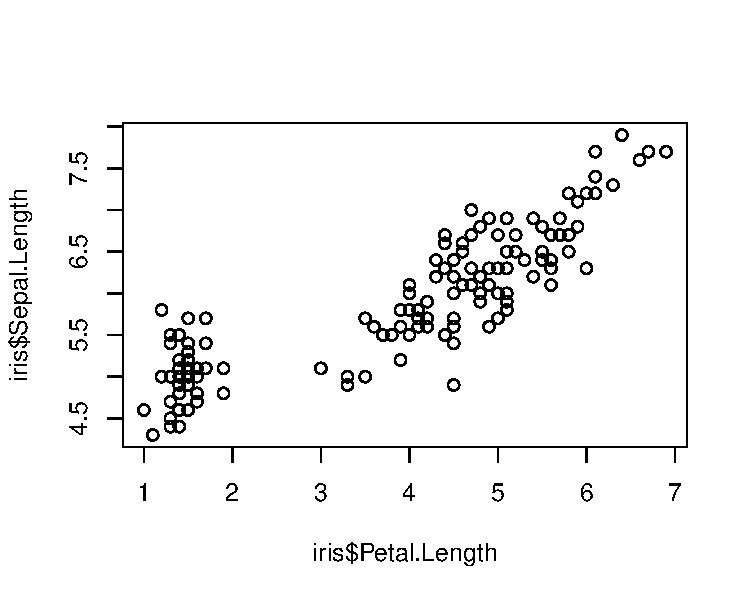
\includegraphics[width=.7\linewidth,height=.6\linewidth]{figure/unnamed-chunk-6-1} 

}



\end{knitrout}
\end{frame}

%------------------------------------------------

\begin{frame}[fragile]
\frametitle{Plots of two variables}
\begin{knitrout}\footnotesize
\definecolor{shadecolor}{rgb}{0.969, 0.969, 0.969}\color{fgcolor}\begin{kframe}
\begin{alltt}
\hlcom{# plot numeric, factor}
\hlkwd{plot}\hlstd{(iris}\hlopt{$}\hlstd{Petal.Length, iris}\hlopt{$}\hlstd{Species)}
\end{alltt}
\end{kframe}

{\centering 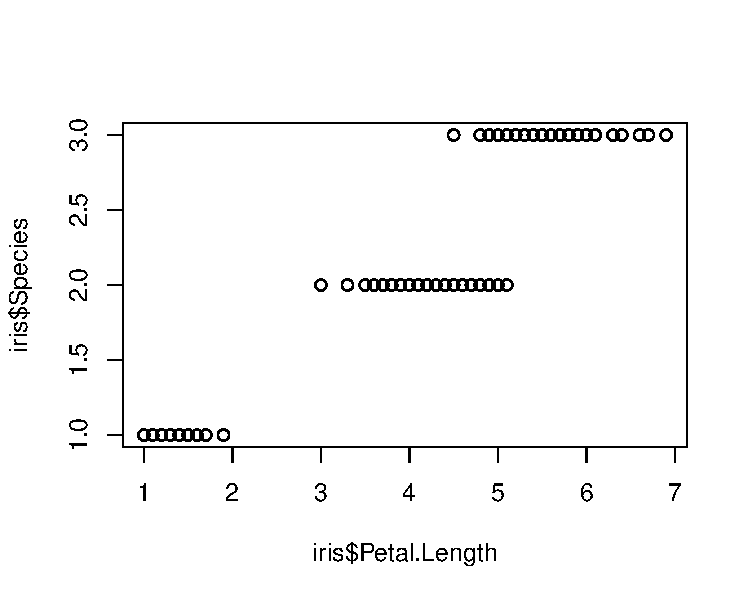
\includegraphics[width=.7\linewidth,height=.6\linewidth]{figure/unnamed-chunk-7-1} 

}



\end{knitrout}
\end{frame}

%------------------------------------------------

\begin{frame}[fragile]
\frametitle{Plots of two variables}
\begin{knitrout}\footnotesize
\definecolor{shadecolor}{rgb}{0.969, 0.969, 0.969}\color{fgcolor}\begin{kframe}
\begin{alltt}
\hlcom{# plot factor, numeric}
\hlkwd{plot}\hlstd{(iris}\hlopt{$}\hlstd{Species, iris}\hlopt{$}\hlstd{Petal.Length)}
\end{alltt}
\end{kframe}

{\centering 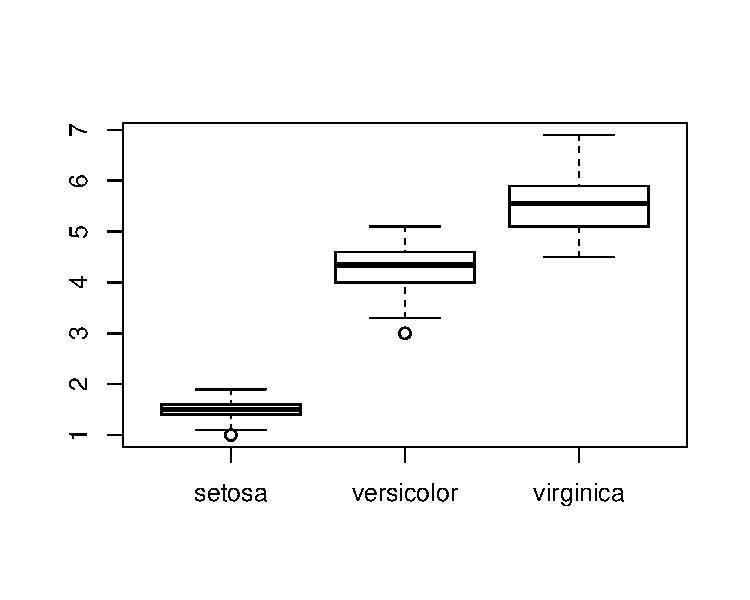
\includegraphics[width=.7\linewidth,height=.6\linewidth]{figure/unnamed-chunk-8-1} 

}



\end{knitrout}
\end{frame}

%------------------------------------------------

\begin{frame}[fragile]
\frametitle{Plots of two variables}
\begin{knitrout}\footnotesize
\definecolor{shadecolor}{rgb}{0.969, 0.969, 0.969}\color{fgcolor}\begin{kframe}
\begin{alltt}
\hlcom{# plot factor, factor}
\hlkwd{plot}\hlstd{(iris}\hlopt{$}\hlstd{Species, iris}\hlopt{$}\hlstd{Species)}
\end{alltt}
\end{kframe}

{\centering 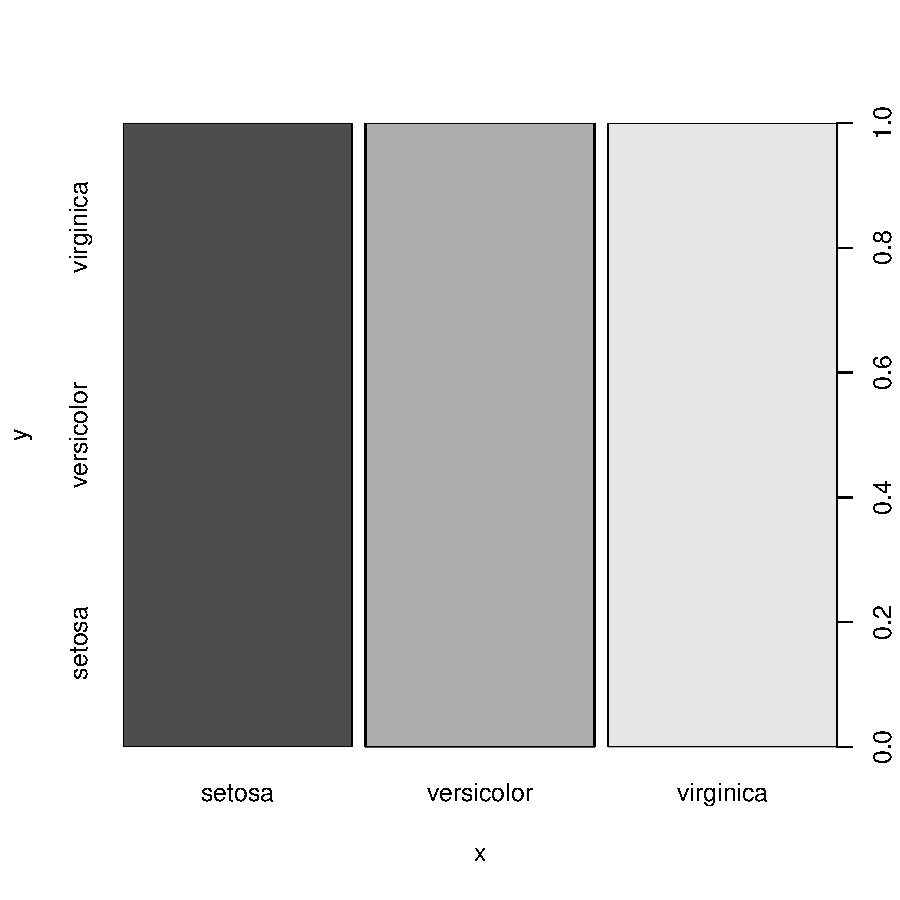
\includegraphics[width=.7\linewidth,height=.6\linewidth]{figure/unnamed-chunk-9-1} 

}



\end{knitrout}
\end{frame}

%------------------------------------------------

\begin{frame}[fragile]
\frametitle{Plots of two variables}
\begin{knitrout}\footnotesize
\definecolor{shadecolor}{rgb}{0.969, 0.969, 0.969}\color{fgcolor}\begin{kframe}
\begin{alltt}
\hlcom{# some fake data}
\hlkwd{set.seed}\hlstd{(}\hlnum{1}\hlstd{)}

\hlcom{# hair color}
\hlstd{hair} \hlkwb{<-} \hlkwd{factor}\hlstd{(}
  \hlkwd{sample}\hlstd{(}\hlkwd{c}\hlstd{(}\hlstr{'blond'}\hlstd{,} \hlstr{'black'}\hlstd{,} \hlstr{'brown'}\hlstd{),} \hlnum{100}\hlstd{,} \hlkwc{replace} \hlstd{=} \hlnum{TRUE}\hlstd{))}

\hlcom{# eye color}
\hlstd{eye} \hlkwb{<-} \hlkwd{factor}\hlstd{(}
  \hlkwd{sample}\hlstd{(}\hlkwd{c}\hlstd{(}\hlstr{'blue'}\hlstd{,} \hlstr{'brown'}\hlstd{,} \hlstr{'green'}\hlstd{),} \hlnum{100}\hlstd{,} \hlkwc{replace} \hlstd{=} \hlnum{TRUE}\hlstd{))}
\end{alltt}
\end{kframe}
\end{knitrout}

\end{frame}

%------------------------------------------------

\begin{frame}[fragile]
\frametitle{Plots of two variables}
\begin{knitrout}\footnotesize
\definecolor{shadecolor}{rgb}{0.969, 0.969, 0.969}\color{fgcolor}\begin{kframe}
\begin{alltt}
\hlcom{# plot factor, factor}
\hlkwd{plot}\hlstd{(hair, eye)}
\end{alltt}
\end{kframe}

{\centering 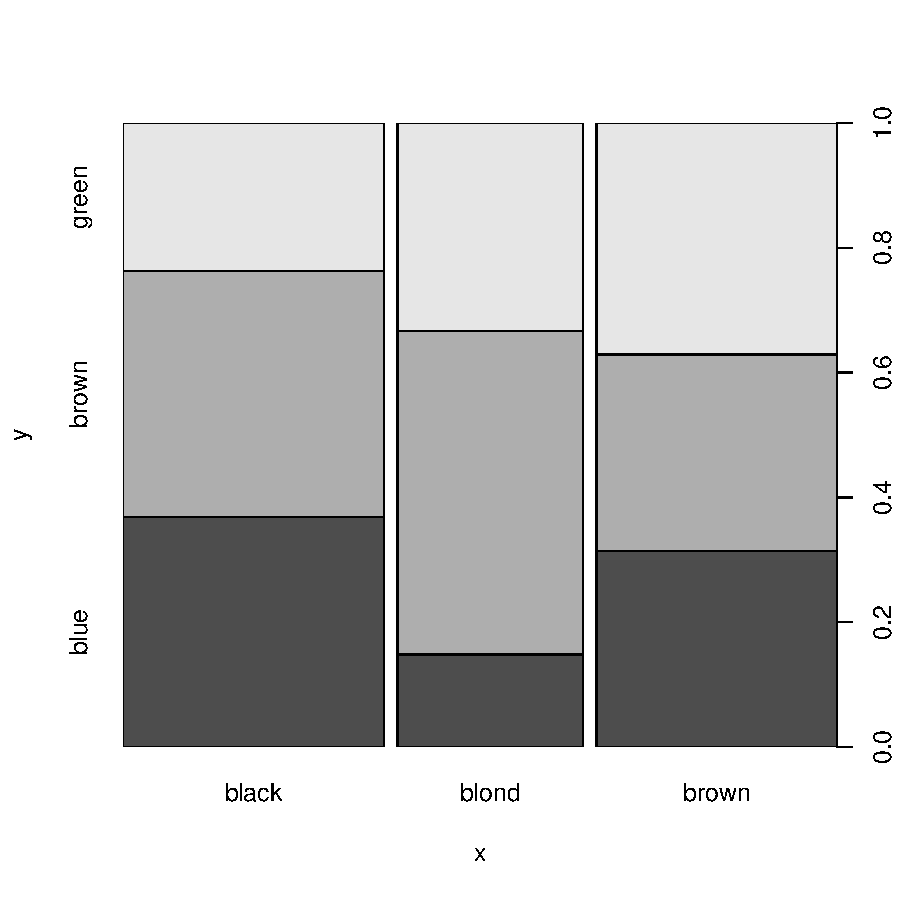
\includegraphics[width=.7\linewidth,height=.6\linewidth]{figure/unnamed-chunk-11-1} 

}



\end{knitrout}
\end{frame}

%------------------------------------------------

\begin{frame}
\frametitle{More high-level graphics of two variables}

{\footnotesize
\begin{center}
 \begin{tabular}{l l l}
  \hline
   Function & Data & Description \\
  \hline
  \code{sunflowerplot()} & numeric, numeric & sunflower scatterplot \\
  \code{smoothScatter()} & numeric, numeric & smooth scatterplot \\
   & & \\
  \code{boxplot()} & list of numeric & boxplots \\
  \code{barplot()} & matrix & stacked / side-by-side barplot  \\
  \code{dotchart()} & matrix & dotplot \\
   & & \\
  \code{stripchart()} & list of numeric & stripcharts \\
  \code{spineplot()} & numeric, factor & spinogram  \\
  \code{cdplot()} & numeric, factor & conditional density plot  \\
   & & \\
  \code{fourfoldplot()} & 2x2 table & fourfold display \\
  \code{assocplot()} & 2-D table & association plot \\  
  \code{mosaicplot()} & 2-D table & mosaic plot \\
  \hline
 \end{tabular}
\end{center}
}

\end{frame}

%------------------------------------------------

\begin{frame}[fragile]
\frametitle{Plots of two variables}
\begin{knitrout}\footnotesize
\definecolor{shadecolor}{rgb}{0.969, 0.969, 0.969}\color{fgcolor}\begin{kframe}
\begin{alltt}
\hlcom{# sunflower plot (numeric, numeric)}
\hlkwd{sunflowerplot}\hlstd{(iris}\hlopt{$}\hlstd{Petal.Length, iris}\hlopt{$}\hlstd{Sepal.Length)}
\end{alltt}
\end{kframe}

{\centering 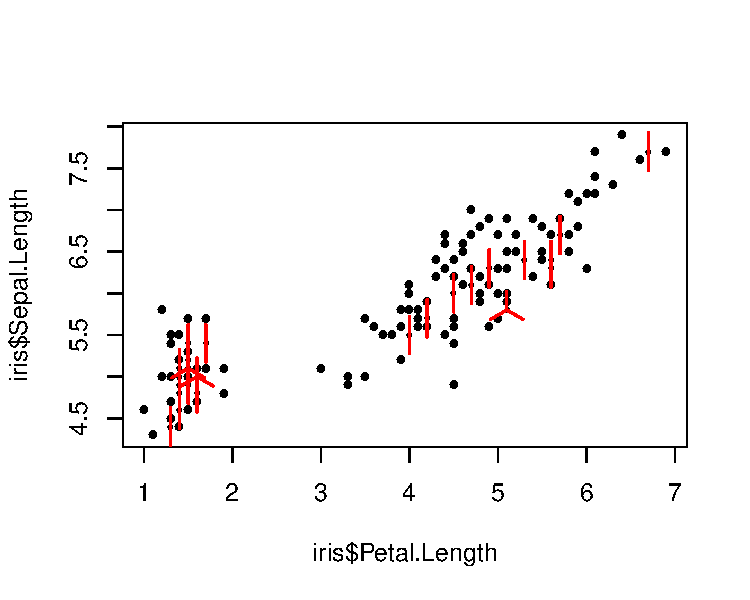
\includegraphics[width=.7\linewidth,height=.6\linewidth]{figure/unnamed-chunk-12-1} 

}



\end{knitrout}
\end{frame}

%------------------------------------------------

\begin{frame}[fragile]
\frametitle{Plots of two variables}
\begin{knitrout}\footnotesize
\definecolor{shadecolor}{rgb}{0.969, 0.969, 0.969}\color{fgcolor}\begin{kframe}
\begin{alltt}
\hlcom{# smooth scatter plot (numeric, numeric)}
\hlkwd{smoothScatter}\hlstd{(iris}\hlopt{$}\hlstd{Petal.Length, iris}\hlopt{$}\hlstd{Sepal.Length)}
\end{alltt}
\end{kframe}

{\centering 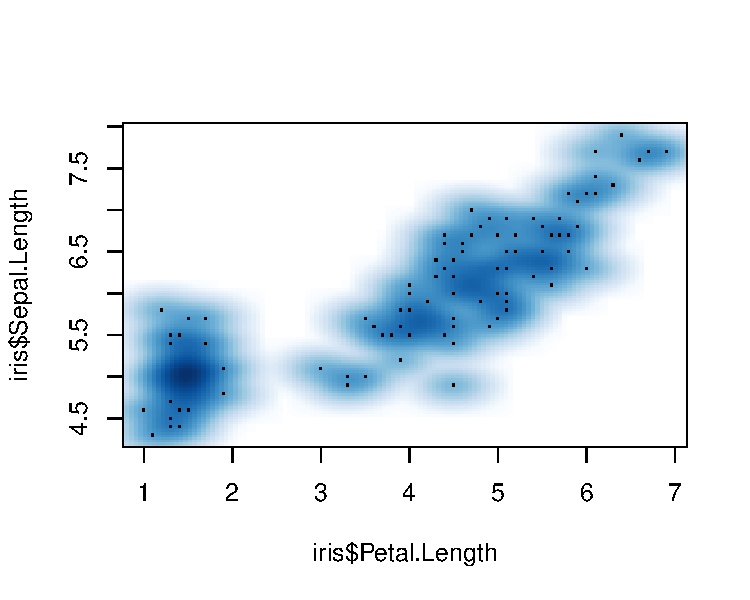
\includegraphics[width=.7\linewidth,height=.6\linewidth]{figure/unnamed-chunk-13-1} 

}



\end{knitrout}
\end{frame}

%------------------------------------------------

\begin{frame}[fragile]
\frametitle{Plots of two variables}
\begin{knitrout}\footnotesize
\definecolor{shadecolor}{rgb}{0.969, 0.969, 0.969}\color{fgcolor}\begin{kframe}
\begin{alltt}
\hlcom{# boxplots (numeric, numeric)}
\hlkwd{boxplot}\hlstd{(iris}\hlopt{$}\hlstd{Petal.Length, iris}\hlopt{$}\hlstd{Sepal.Length)}
\end{alltt}
\end{kframe}

{\centering 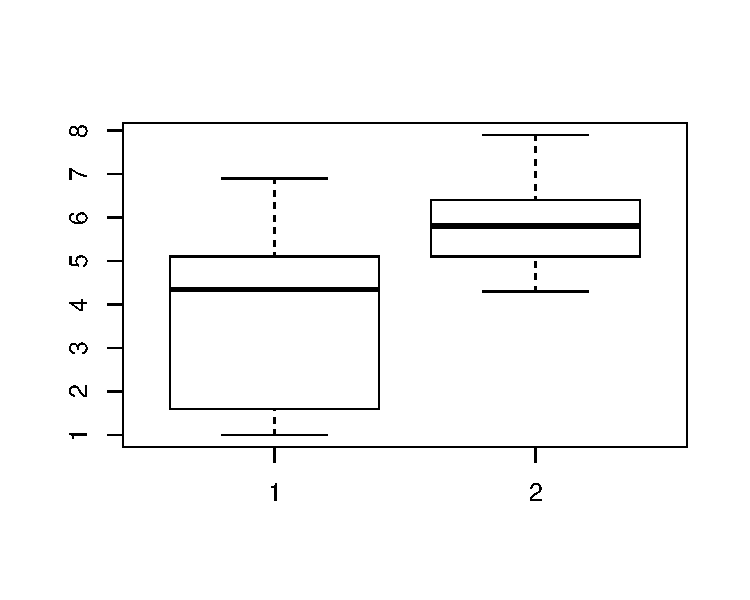
\includegraphics[width=.7\linewidth,height=.6\linewidth]{figure/unnamed-chunk-14-1} 

}



\end{knitrout}
\end{frame}

%------------------------------------------------

\begin{frame}[fragile]
\frametitle{Plots of two variables}
\begin{knitrout}\footnotesize
\definecolor{shadecolor}{rgb}{0.969, 0.969, 0.969}\color{fgcolor}\begin{kframe}
\begin{alltt}
\hlstd{m} \hlkwb{<-} \hlkwd{matrix}\hlstd{(}\hlnum{1}\hlopt{:}\hlnum{8}\hlstd{,} \hlnum{4}\hlstd{,} \hlnum{2}\hlstd{)}
\hlcom{# barplot (numeric matrix)}
\hlkwd{barplot}\hlstd{(m)}
\end{alltt}
\end{kframe}

{\centering 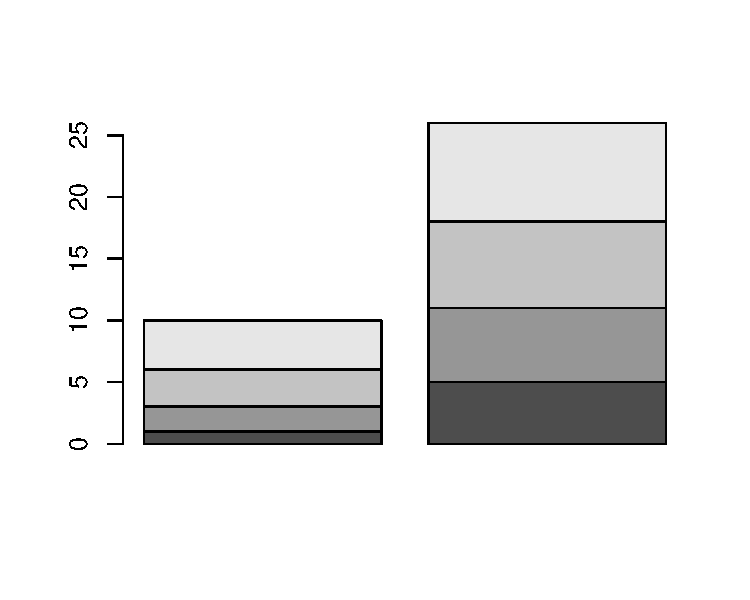
\includegraphics[width=.7\linewidth,height=.6\linewidth]{figure/unnamed-chunk-15-1} 

}



\end{knitrout}
\end{frame}

%------------------------------------------------

\begin{frame}[fragile]
\frametitle{Plots of two variables}
\begin{knitrout}\footnotesize
\definecolor{shadecolor}{rgb}{0.969, 0.969, 0.969}\color{fgcolor}\begin{kframe}
\begin{alltt}
\hlstd{m} \hlkwb{<-} \hlkwd{matrix}\hlstd{(}\hlnum{1}\hlopt{:}\hlnum{8}\hlstd{,} \hlnum{4}\hlstd{,} \hlnum{2}\hlstd{)}
\hlcom{# barplot (numeric matrix)}
\hlkwd{barplot}\hlstd{(m,} \hlkwc{beside} \hlstd{=} \hlnum{TRUE}\hlstd{)}
\end{alltt}
\end{kframe}

{\centering 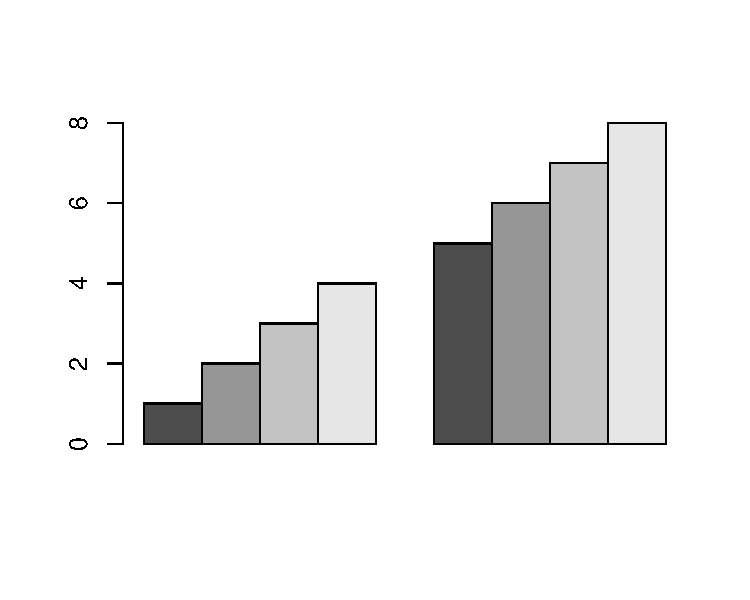
\includegraphics[width=.7\linewidth,height=.6\linewidth]{figure/unnamed-chunk-16-1} 

}



\end{knitrout}
\end{frame}

%------------------------------------------------

\begin{frame}[fragile]
\frametitle{Plots of two variables}
\begin{knitrout}\footnotesize
\definecolor{shadecolor}{rgb}{0.969, 0.969, 0.969}\color{fgcolor}\begin{kframe}
\begin{alltt}
\hlcom{# conditional density plot (numeric, factor)}
\hlkwd{cdplot}\hlstd{(iris}\hlopt{$}\hlstd{Petal.Length, iris}\hlopt{$}\hlstd{Species)}
\end{alltt}
\end{kframe}

{\centering 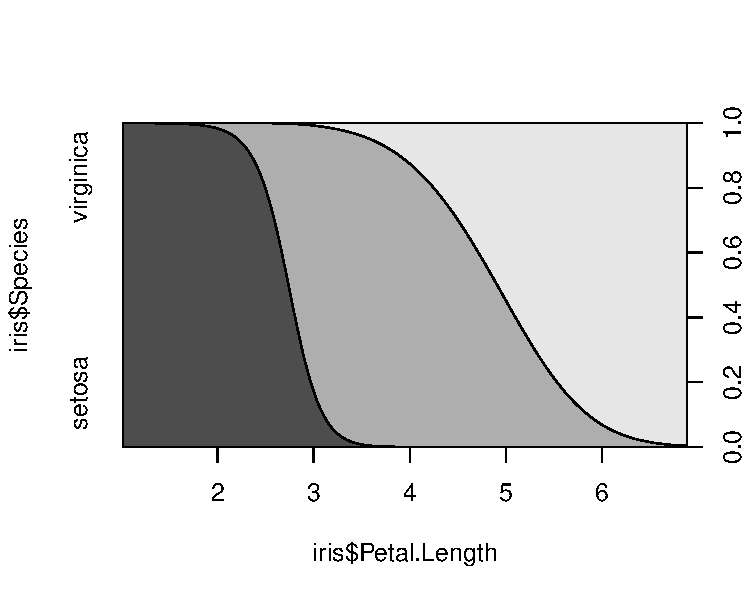
\includegraphics[width=.7\linewidth,height=.6\linewidth]{figure/unnamed-chunk-17-1} 

}



\end{knitrout}
\end{frame}

%------------------------------------------------

\begin{frame}[fragile]
\frametitle{Two categorical variables: frequency table}
\begin{knitrout}\footnotesize
\definecolor{shadecolor}{rgb}{0.969, 0.969, 0.969}\color{fgcolor}\begin{kframe}
\begin{alltt}
\hlcom{# 2-D table (HairEyeColor data)}
\hlstd{x} \hlkwb{<-} \hlkwd{margin.table}\hlstd{(HairEyeColor,} \hlkwd{c}\hlstd{(}\hlnum{1}\hlstd{,} \hlnum{2}\hlstd{))}
\hlstd{x}
\end{alltt}
\begin{verbatim}
##        Eye
## Hair    Brown Blue Hazel Green
##   Black    68   20    15     5
##   Brown   119   84    54    29
##   Red      26   17    14    14
##   Blond     7   94    10    16
\end{verbatim}
\end{kframe}
\end{knitrout}
\end{frame}

%------------------------------------------------

\begin{frame}[fragile]
\frametitle{Plots of two categorical variables}
\begin{knitrout}\footnotesize
\definecolor{shadecolor}{rgb}{0.969, 0.969, 0.969}\color{fgcolor}\begin{kframe}
\begin{alltt}
\hlcom{# mosaic plot (2-D table)}
\hlkwd{mosaicplot}\hlstd{(x,} \hlkwc{main} \hlstd{=} \hlstr{"Relation between hair and eye color"}\hlstd{)}
\end{alltt}
\end{kframe}

{\centering 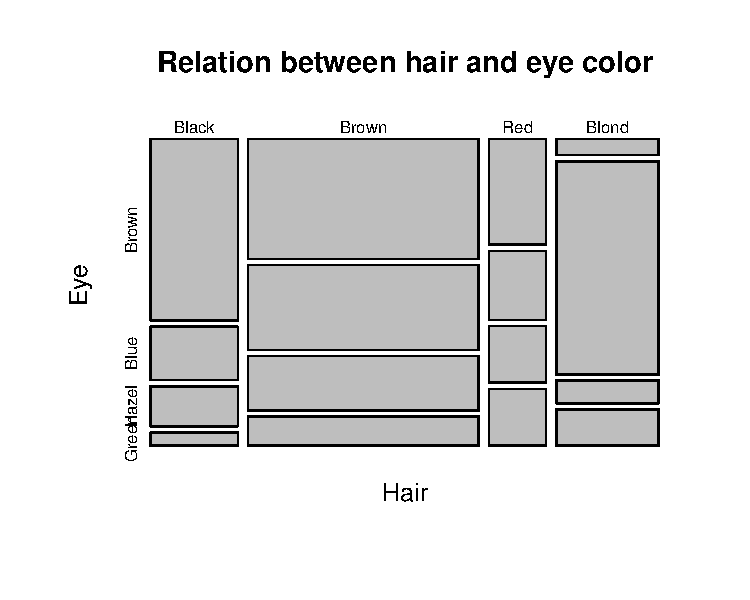
\includegraphics[width=.7\linewidth,height=.6\linewidth]{figure/unnamed-chunk-19-1} 

}



\end{knitrout}
\end{frame}

%------------------------------------------------

\begin{frame}[fragile]
\frametitle{Plots of two categorical variables}
\begin{knitrout}\footnotesize
\definecolor{shadecolor}{rgb}{0.969, 0.969, 0.969}\color{fgcolor}\begin{kframe}
\begin{alltt}
\hlcom{# association plot (2-D table)}
\hlkwd{assocplot}\hlstd{(x,} \hlkwc{main} \hlstd{=} \hlstr{"Relation between hair and eye color"}\hlstd{)}
\end{alltt}
\end{kframe}

{\centering 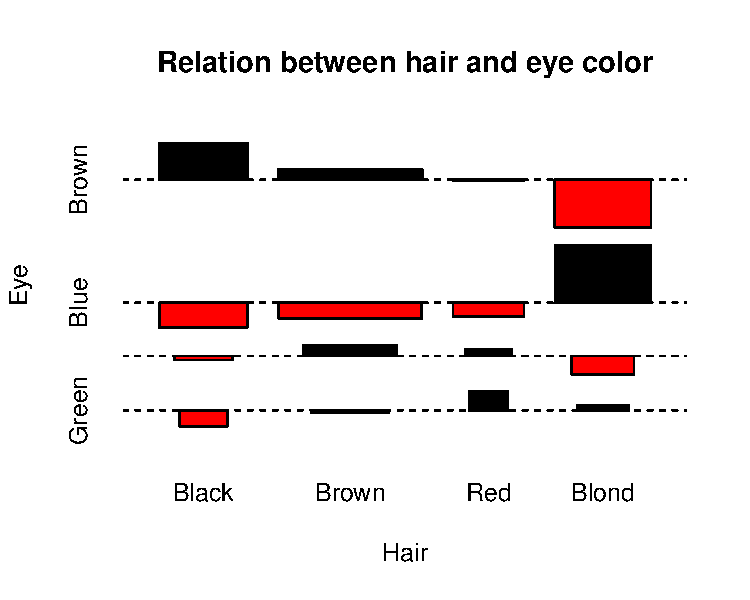
\includegraphics[width=.7\linewidth,height=.6\linewidth]{figure/unnamed-chunk-20-1} 

}



\end{knitrout}
\end{frame}

%------------------------------------------------

\begin{frame}
\begin{center}
\Huge{\hilit{Plots of Multiple Variables}}
\end{center}
\end{frame}

%------------------------------------------------

\begin{frame}
\frametitle{High-level graphics of multiple variables}

{\footnotesize
\begin{center}
 \begin{tabular}{l l l}
  \hline
   Function & Data & Description \\
  \hline
  \code{plot()} & data frame & scatterplot matrix \\
  \code{pairs()} & matrix & scatterplot matrix \\
  \code{matplot()} & matrix & scatterplot \\
  \code{stars()} & matrix & star plots \\
   & & \\
  \code{image()} & numeric, numeric, numeric & image plot \\
  \code{contour()} & numeric, numeric, numeric & contour plot  \\
  \code{filled.contour()} & numeric, numeric, numeric & filled contour plot  \\
  \code{persp()} & numeric, numeric, numeric & 3-D surface \\
  \code{symbols()} & numeric, numeric, numeric & symbols scatterplot \\
   & & \\
  \code{mosaicplot()} & N-D table & mosaic plot \\
  \hline
 \end{tabular}
\end{center}
}

\end{frame}

%------------------------------------------------

\begin{frame}[fragile]
\frametitle{Plots of multiple variables}
\begin{knitrout}\footnotesize
\definecolor{shadecolor}{rgb}{0.969, 0.969, 0.969}\color{fgcolor}\begin{kframe}
\begin{alltt}
\hlcom{# scatter plot matrix (data frame)}
\hlkwd{plot}\hlstd{(iris[ ,} \hlnum{1}\hlopt{:}\hlnum{4}\hlstd{])}
\end{alltt}
\end{kframe}

{\centering 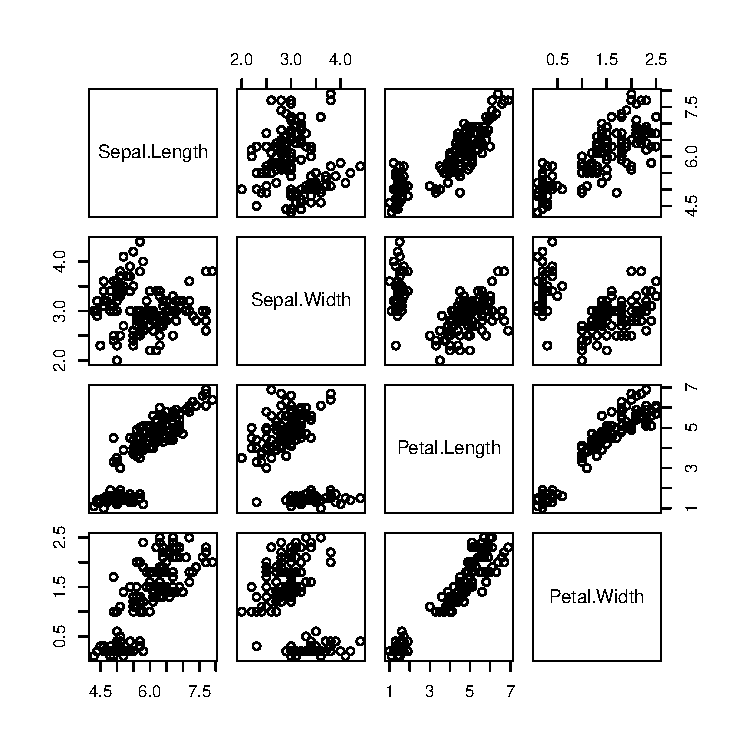
\includegraphics[width=.6\linewidth,height=.6\linewidth]{figure/unnamed-chunk-21-1} 

}



\end{knitrout}
\end{frame}

%------------------------------------------------

\begin{frame}[fragile]
\frametitle{Plots of multiple variables}
\begin{knitrout}\footnotesize
\definecolor{shadecolor}{rgb}{0.969, 0.969, 0.969}\color{fgcolor}\begin{kframe}
\begin{alltt}
\hlcom{# scatter plot matrix (data frame)}
\hlkwd{pairs}\hlstd{(iris[ ,} \hlnum{1}\hlopt{:}\hlnum{4}\hlstd{])}
\end{alltt}
\end{kframe}

{\centering 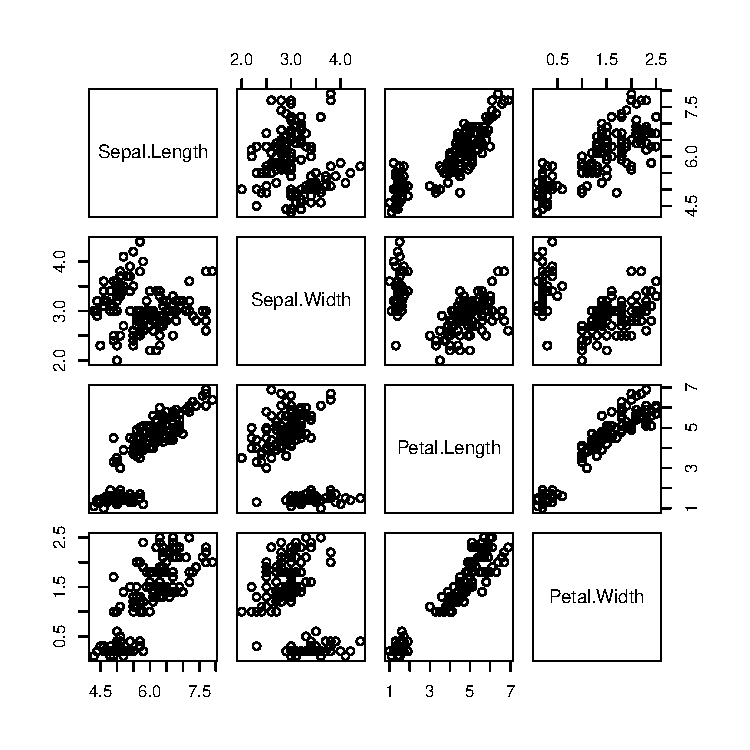
\includegraphics[width=.6\linewidth,height=.6\linewidth]{figure/unnamed-chunk-22-1} 

}



\end{knitrout}
\end{frame}

%------------------------------------------------

\begin{frame}[fragile]
\frametitle{Plots of multiple variables}
\begin{knitrout}\footnotesize
\definecolor{shadecolor}{rgb}{0.969, 0.969, 0.969}\color{fgcolor}\begin{kframe}
\begin{alltt}
\hlcom{# scatter plot matrix (data frame)}
\hlkwd{matplot}\hlstd{(iris[ ,} \hlnum{1}\hlopt{:}\hlnum{4}\hlstd{])}
\end{alltt}
\end{kframe}

{\centering 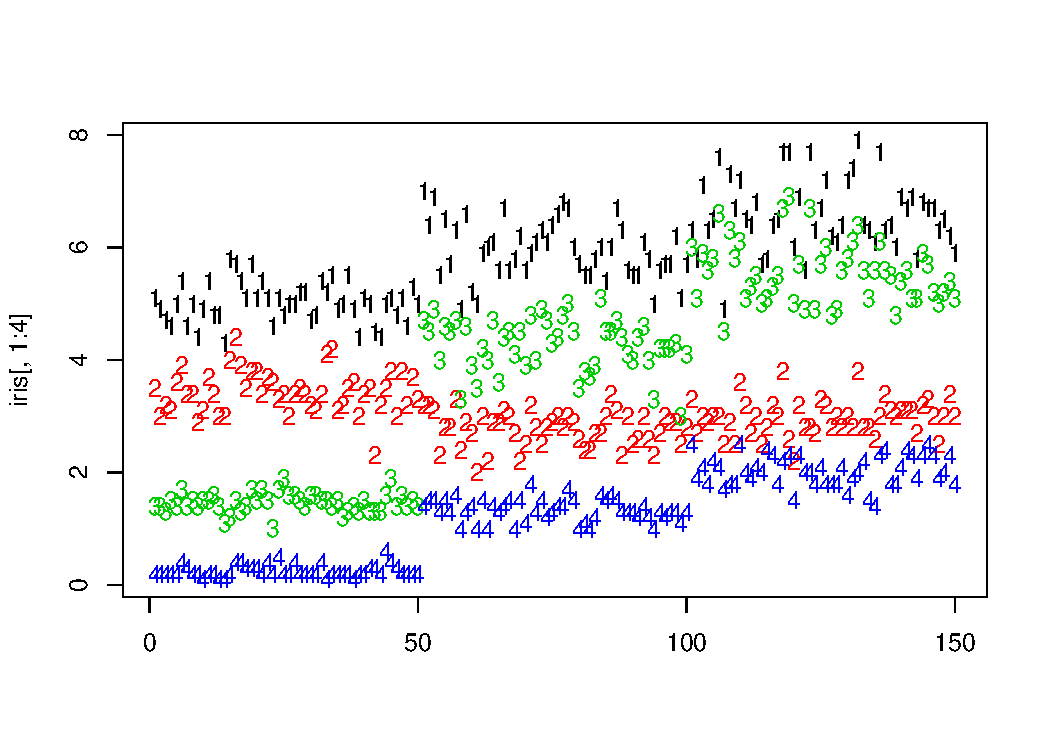
\includegraphics[width=.8\linewidth,height=.65\linewidth]{figure/unnamed-chunk-23-1} 

}



\end{knitrout}
\end{frame}

%------------------------------------------------

\begin{frame}[fragile]
\frametitle{Plots of multiple variables}
\begin{knitrout}\footnotesize
\definecolor{shadecolor}{rgb}{0.969, 0.969, 0.969}\color{fgcolor}\begin{kframe}
\begin{alltt}
\hlcom{# star plot (data frame)}
\hlkwd{stars}\hlstd{(iris[ ,} \hlnum{1}\hlopt{:}\hlnum{4}\hlstd{])}
\end{alltt}
\end{kframe}

{\centering 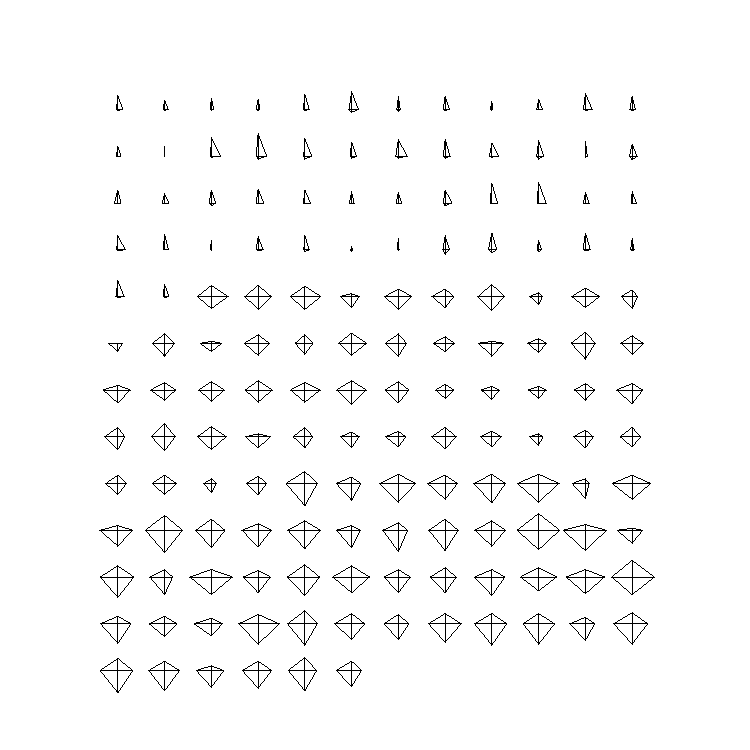
\includegraphics[width=.6\linewidth,height=.6\linewidth]{figure/unnamed-chunk-24-1} 

}



\end{knitrout}
\end{frame}

%------------------------------------------------

\begin{frame}[fragile]
\frametitle{Plots of multiple variables}
\begin{knitrout}\footnotesize
\definecolor{shadecolor}{rgb}{0.969, 0.969, 0.969}\color{fgcolor}\begin{kframe}
\begin{alltt}
\hlcom{# color image (matrix)}
\hlkwd{image}\hlstd{(}\hlkwd{t}\hlstd{(volcano)[}\hlkwd{ncol}\hlstd{(volcano)}\hlopt{:}\hlnum{1}\hlstd{, ])}
\end{alltt}
\end{kframe}

{\centering 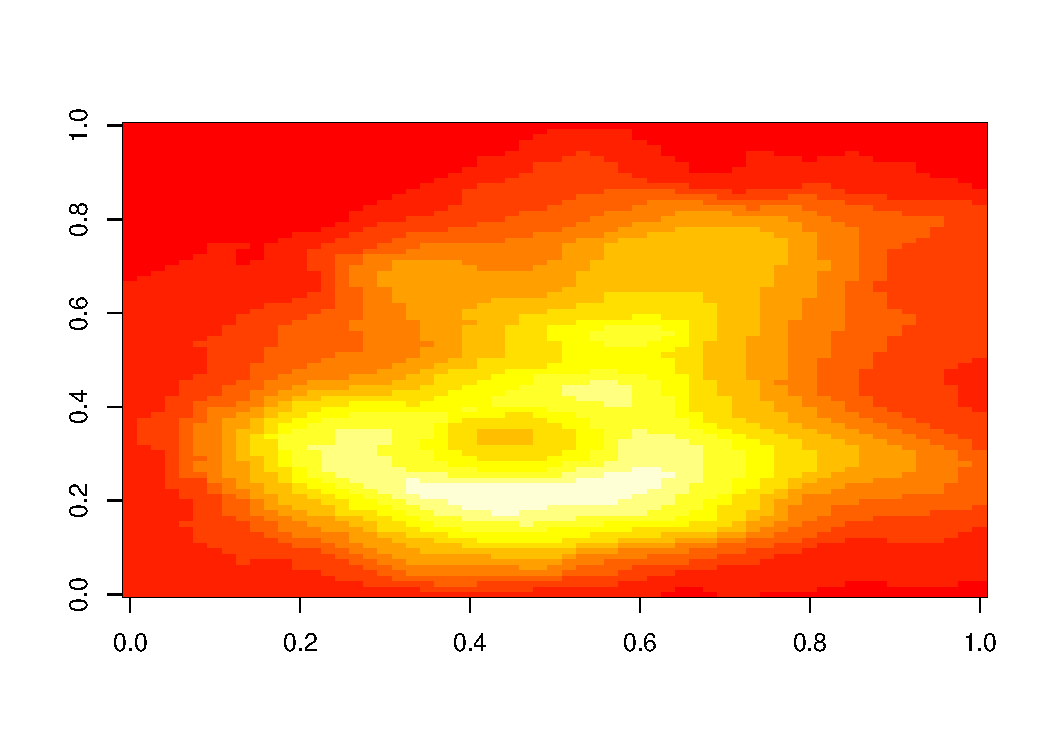
\includegraphics[width=.8\linewidth,height=.65\linewidth]{figure/unnamed-chunk-25-1} 

}



\end{knitrout}
\end{frame}

%------------------------------------------------

\begin{frame}[fragile]
\frametitle{Plots of multiple variables}
\begin{knitrout}\footnotesize
\definecolor{shadecolor}{rgb}{0.969, 0.969, 0.969}\color{fgcolor}\begin{kframe}
\begin{alltt}
\hlcom{# display of Maunga Whau volcano}
\hlstd{x} \hlkwb{<-} \hlnum{10}\hlopt{*}\hlstd{(}\hlnum{1}\hlopt{:}\hlkwd{nrow}\hlstd{(volcano))}
\hlstd{y} \hlkwb{<-} \hlnum{10}\hlopt{*}\hlstd{(}\hlnum{1}\hlopt{:}\hlkwd{ncol}\hlstd{(volcano))}
\hlkwd{image}\hlstd{(x, y, volcano,} \hlkwc{col} \hlstd{=} \hlkwd{terrain.colors}\hlstd{(}\hlnum{100}\hlstd{),} \hlkwc{axes} \hlstd{=} \hlnum{FALSE}\hlstd{)}
\hlkwd{contour}\hlstd{(x, y, volcano,} \hlkwc{levels} \hlstd{=} \hlkwd{seq}\hlstd{(}\hlnum{90}\hlstd{,} \hlnum{200}\hlstd{,} \hlkwc{by} \hlstd{=} \hlnum{5}\hlstd{),}
        \hlkwc{add} \hlstd{=} \hlnum{TRUE}\hlstd{,} \hlkwc{col} \hlstd{=} \hlstr{"peru"}\hlstd{)}
\hlkwd{axis}\hlstd{(}\hlnum{1}\hlstd{,} \hlkwc{at} \hlstd{=} \hlkwd{seq}\hlstd{(}\hlnum{100}\hlstd{,} \hlnum{800}\hlstd{,} \hlkwc{by} \hlstd{=} \hlnum{100}\hlstd{))}
\hlkwd{axis}\hlstd{(}\hlnum{2}\hlstd{,} \hlkwc{at} \hlstd{=} \hlkwd{seq}\hlstd{(}\hlnum{100}\hlstd{,} \hlnum{600}\hlstd{,} \hlkwc{by} \hlstd{=} \hlnum{100}\hlstd{))}
\hlkwd{box}\hlstd{()}
\hlkwd{title}\hlstd{(}\hlkwc{main} \hlstd{=} \hlstr{"Maunga Whau Volcano"}\hlstd{,} \hlkwc{font.main} \hlstd{=} \hlnum{4}\hlstd{)}
\end{alltt}
\end{kframe}
\end{knitrout}
\end{frame}

%------------------------------------------------

\begin{frame}[fragile]
\frametitle{Plots of multiple variables}
\begin{knitrout}\footnotesize
\definecolor{shadecolor}{rgb}{0.969, 0.969, 0.969}\color{fgcolor}

{\centering 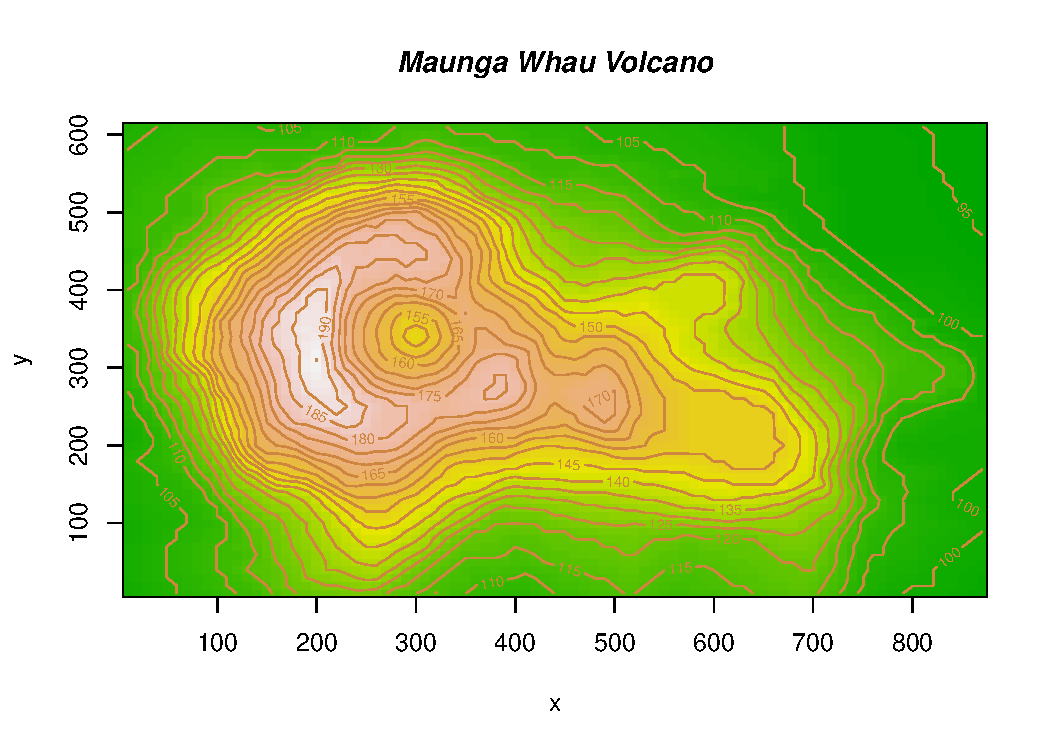
\includegraphics[width=.8\linewidth,height=.65\linewidth]{figure/volcano-1} 

}



\end{knitrout}
\end{frame}

%------------------------------------------------

\begin{frame}[fragile]
\frametitle{Plots of multiple variables}
\begin{knitrout}\footnotesize
\definecolor{shadecolor}{rgb}{0.969, 0.969, 0.969}\color{fgcolor}\begin{kframe}
\begin{alltt}
\hlcom{# mosaic plot of N-D tables}
\hlkwd{mosaicplot}\hlstd{(HairEyeColor)}
\end{alltt}
\end{kframe}

{\centering 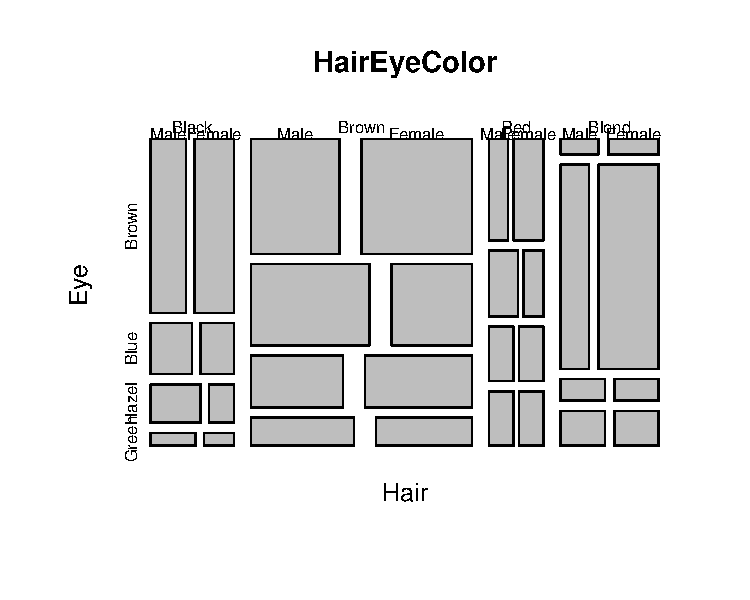
\includegraphics[width=.75\linewidth,height=.65\linewidth]{figure/unnamed-chunk-26-1} 

}



\end{knitrout}
\end{frame}

%------------------------------------------------

\begin{frame}[fragile]
\frametitle{Plots of multiple variables}
\begin{knitrout}\scriptsize
\definecolor{shadecolor}{rgb}{0.969, 0.969, 0.969}\color{fgcolor}\begin{kframe}
\begin{alltt}
\hlcom{# symbols scatter plots}
\hlkwd{symbols}\hlstd{(iris[,} \hlnum{1}\hlstd{], iris[,} \hlnum{2}\hlstd{],} \hlkwc{circles} \hlstd{= iris[,} \hlnum{3}\hlstd{]}\hlopt{/}\hlnum{100}\hlstd{,}
        \hlkwc{inches} \hlstd{=} \hlnum{FALSE}\hlstd{)}
\end{alltt}
\end{kframe}

{\centering 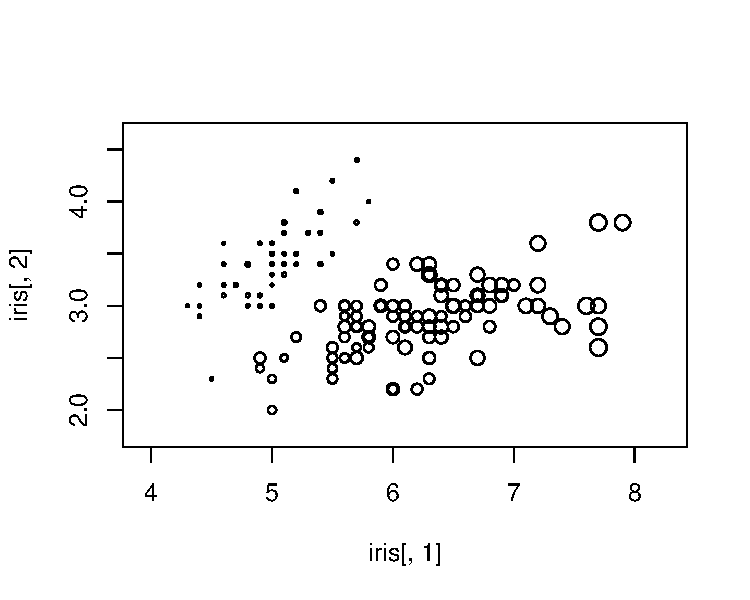
\includegraphics[width=.8\linewidth,height=.65\linewidth]{figure/unnamed-chunk-27-1} 

}



\end{knitrout}
\end{frame}

%------------------------------------------------

\begin{frame}
\frametitle{Graphics Parameters}

\bb{Graphics Functions and Arguments}
\bi
  \item Plot functions usually come with various arguments
  \item Typically, the first argument(s) is the data object(s) to be plotted
  \item Most of the other arguments have default options
  \item Graphic arguments have a consisting naming convention, but there will always be some exception
\ei
\eb

\end{frame}

%------------------------------------------------

\begin{frame}
\frametitle{Graphical Parameters}

\bb{Graphical Arguments}
\bi
  \item Some arguments are specific to a function (e.g. \code{horiz} or \code{beside} in \code{barplot()})
  \item Other arguments are more general (e.g. \code{col}, \code{xlab}, \code{ylab})
  \item General graphical parameters are listed in the documentation of the function {\hilit \code{par()}}
  \item See \code{?par} for more information
\ei
\eb

\end{frame}

%------------------------------------------------

\begin{frame}
\frametitle{Graphics in R}

\bb{How to choose a graphics approach?}
\bi
  \item look first for an existing function that does what you want ---or something similar to what you want (don't reivent the wheel!)
  \item Existing plotting functions can be combined and customized by using optional arguments or graphical parameters
  \item For exploratory data analysis (quick and dirty) the plotting functions in \code{"graphics"} is a good option
\ei
\eb

\end{frame}

%------------------------------------------------


\end{document}
